
\slidesectionwithgraphic{Treemap Categories}{images/white-city-map-cropped.jpg}

\newlength{\examplesdefaultwidth}
\newlength{\exampleslargewidth}
\setlength{\examplesdefaultwidth}{0.17\textwidth} %
\setlength{\exampleslargewidth}{0.39\textwidth} %

\begin{frame}[c]{Splitting Treemap -- \Ts}
	\begin{figure}
		\centering
		\footnotesize
		\begin{tikzpicture}[every node/.style={inner sep=0,outer sep=0},node distance=0pt]
		\node[] (sot-1) {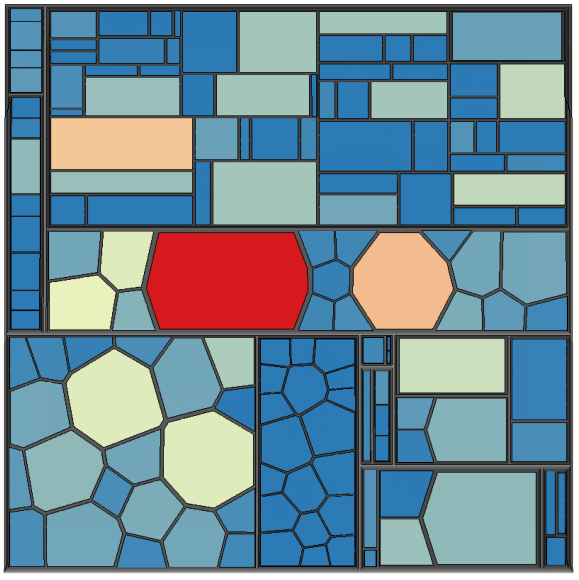
\includegraphics[width=\exampleslargewidth]{figures/mixed-treemap-layouting.png}};
		\node[below=5pt of sot-1,text width=0.7\exampleslargewidth,align=center] (sot-1-label) { Hybrid Layout Treemap };
		\node[right=10pt of sot-1.north east,anchor=north west] (sot-2) {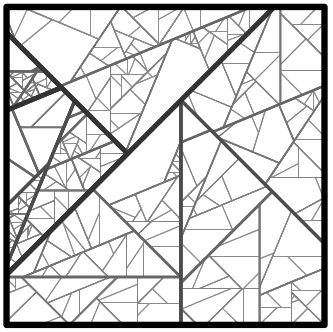
\includegraphics[width=\examplesdefaultwidth]{figures/bound-aspect-ratio.png}};
		\node[below=5pt of sot-2,text width=\examplesdefaultwidth,align=center] (sot-2-label) { Treemap with Bound Aspect Ratio };
		\node[right=10pt of sot-2] (sot-3) {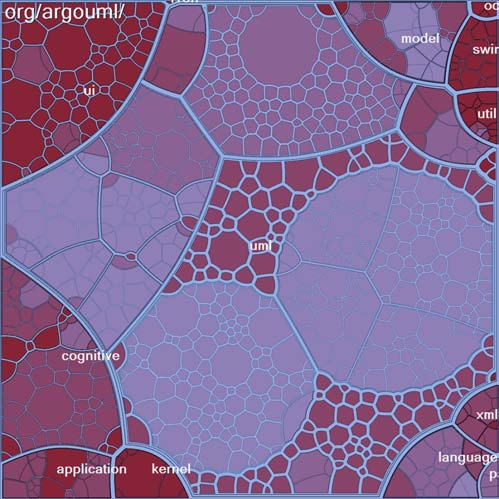
\includegraphics[width=\examplesdefaultwidth]{figures/voronoitreemap.png}};
		\node[below=5pt of sot-3,text width=\examplesdefaultwidth,align=center] (sot-3-label) { Voronoi Treemap };
		\node[right=10pt of sot-1.south east,anchor=south west] (sot-4) {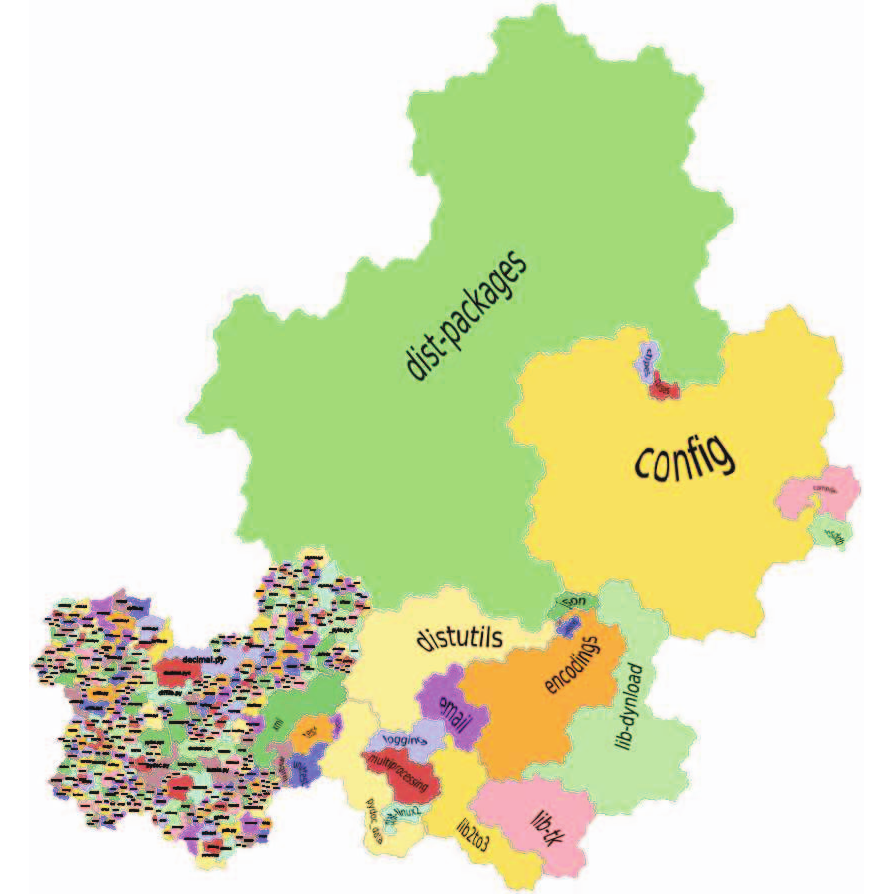
\includegraphics[width=\examplesdefaultwidth]{figures/gospermap.png}};
		\node[below=5pt of sot-4,text width=\examplesdefaultwidth,align=center] (sot-4-label) { GosperMap };
		\node[right=10pt of sot-4] (sot-5) {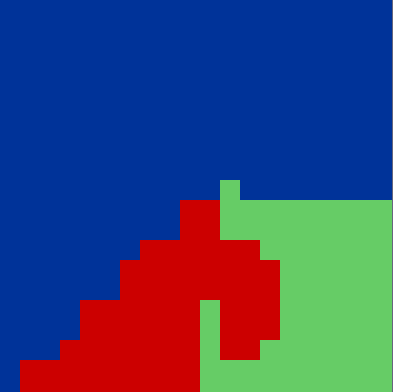
\includegraphics[width=\examplesdefaultwidth]{figures/jigsaw.png}};
		\node[below=5pt of sot-5,text width=\examplesdefaultwidth,align=center] (sot-5-label) { Jigsaw Treemap };
		\node[above=5pt of sot-2.north west,xshift=-5pt] (Ts) { \Ts };
		\draw[thin,black,shorten >= 10pt] (Ts-|sot-1.west) -- (Ts);
		\draw[thin,black,shorten <= 10pt] (Ts) -- (Ts-|sot-3.east);
		\end{tikzpicture}
		\caption{Examples of treemaps from the category \emph{Space-Filling Treemap}. Image courtesy from left to right and top to bottom: \cite{hahn2017-hybrid}, \cite{deBerg2011-bounded}, \cite{balzer2005-softwaremetrics}, \cite{auber2013-gospermap}, and \cite{wattenberg2005-spacefillingcurves}.}
	\end{figure}
\end{frame}

\begin{frame}[c]{Packing Treemap -- \Tc}
	\begin{figure}
		\centering
		\footnotesize
		\begin{tikzpicture}[every node/.style={inner sep=0,outer sep=0},node distance=0pt]
		\node[] (sot-1) {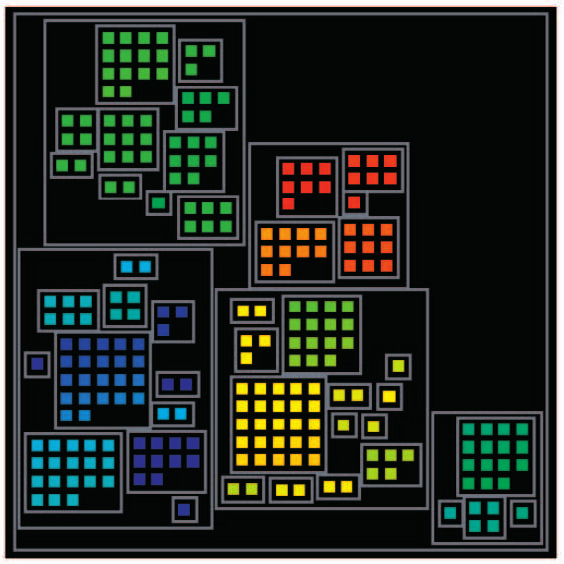
\includegraphics[width=\exampleslargewidth]{figures/data-jewelry-box.png}};
		\node[below=5pt of sot-1,text width=0.7\exampleslargewidth,align=center] (sot-1-label) { Data-Jewelry Box };
		\node[right=10pt of sot-1.north east,anchor=north west] (sot-2) {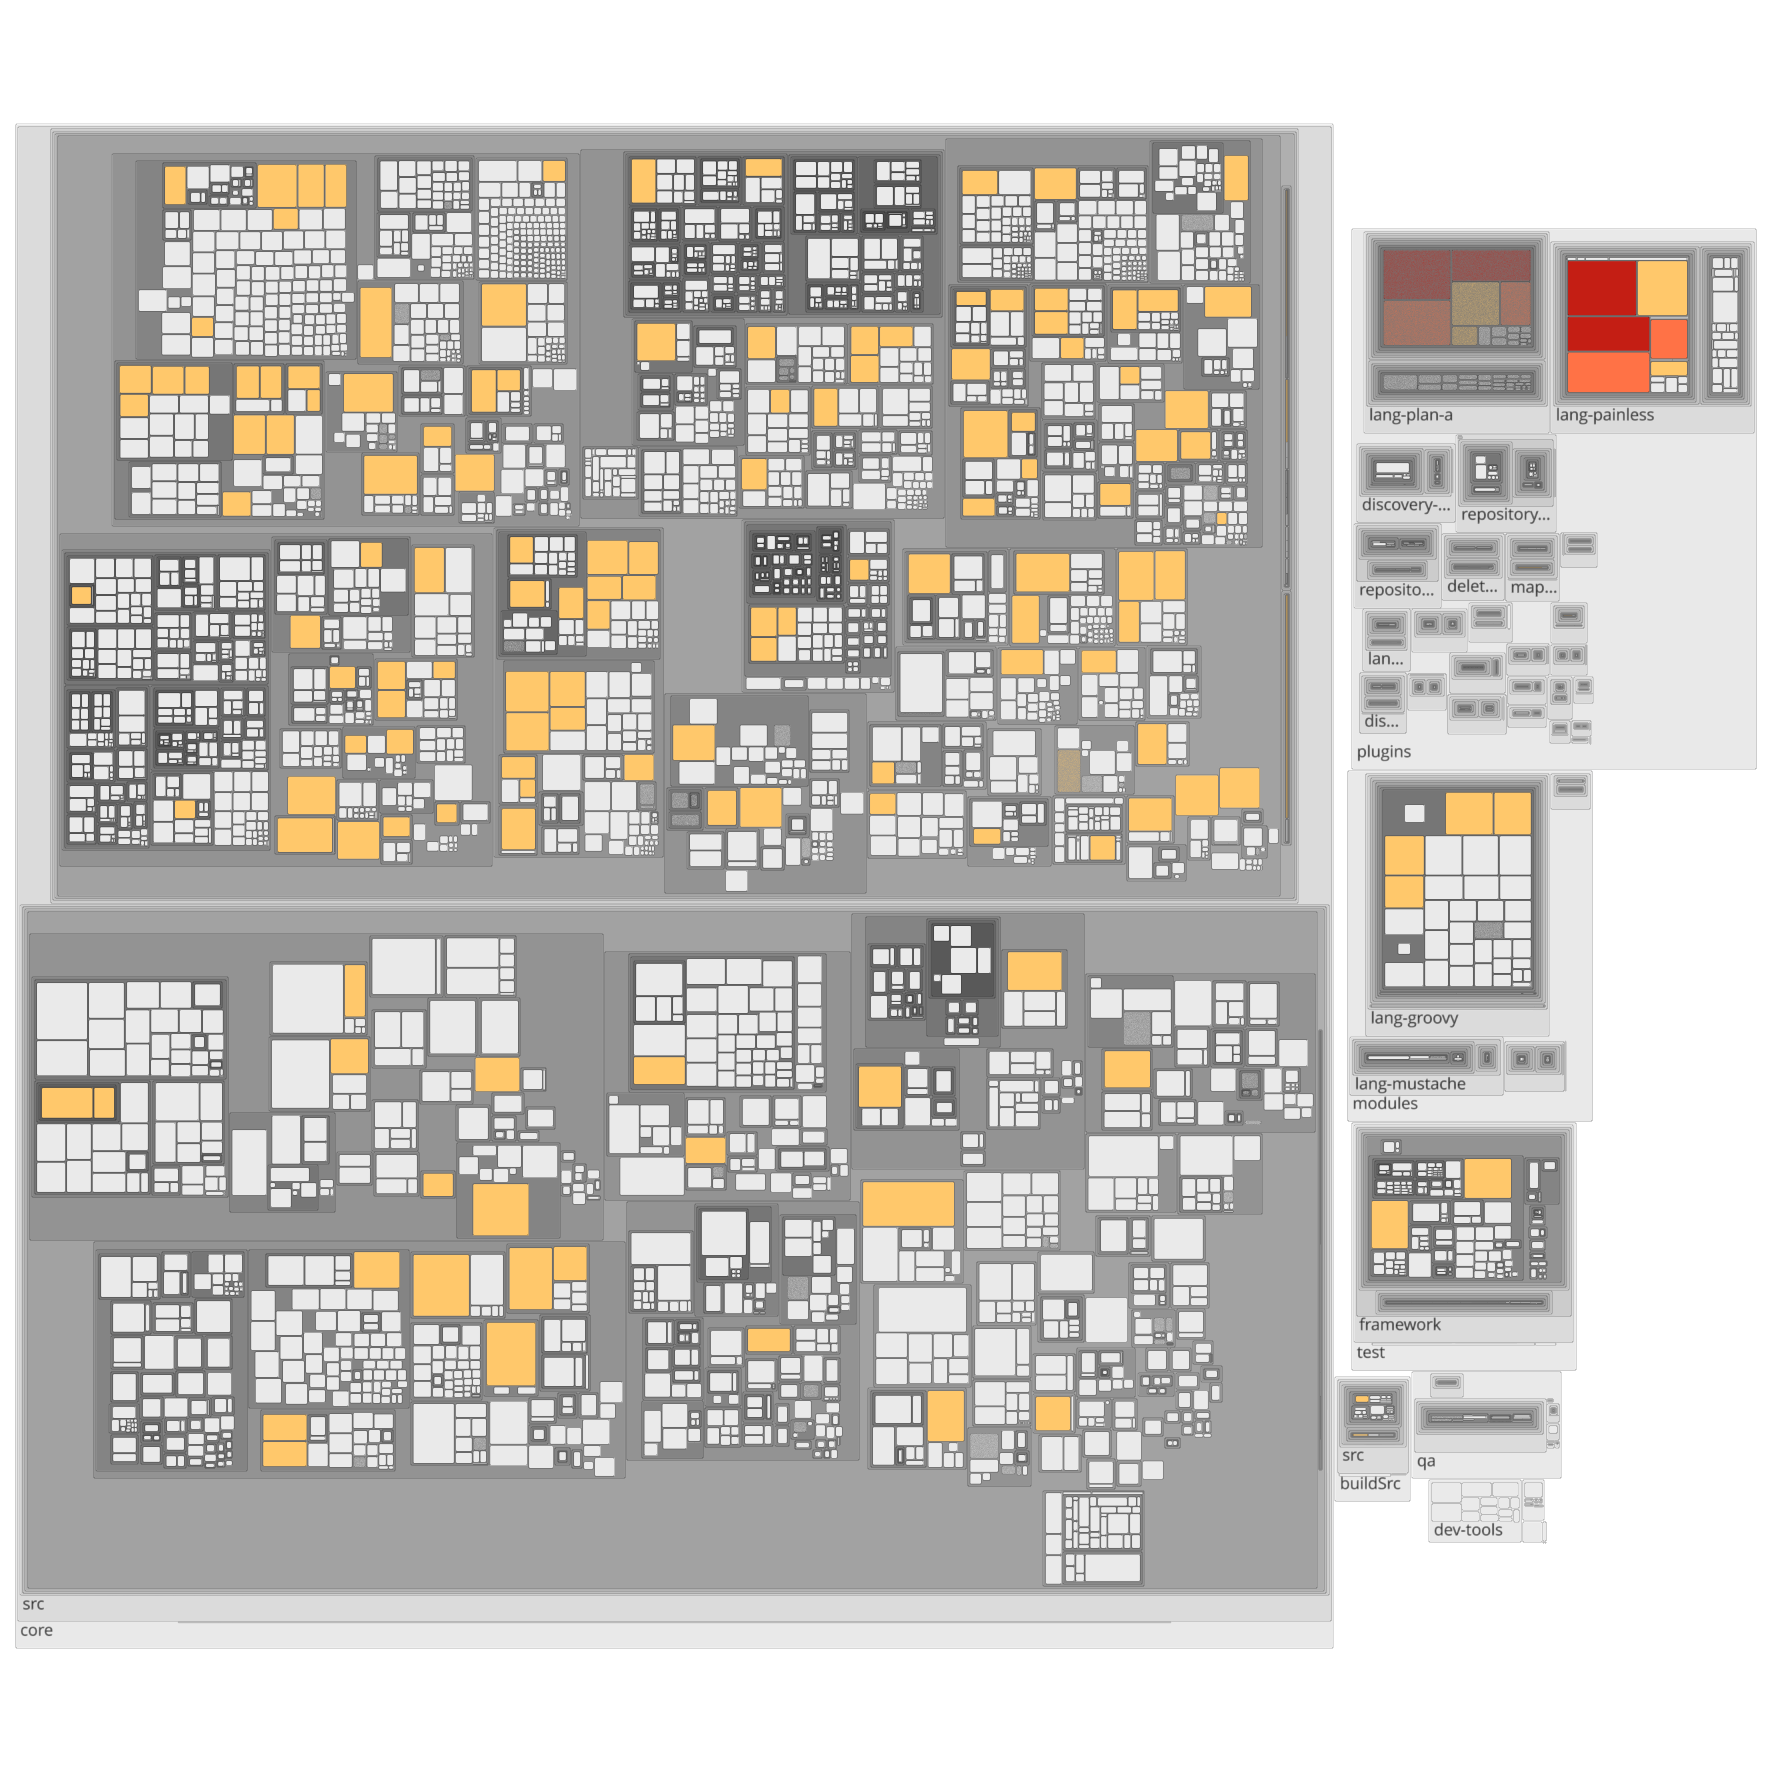
\includegraphics[width=\examplesdefaultwidth]{figures/evocells.png}};
		\node[below=5pt of sot-2,text width=\examplesdefaultwidth,align=center] (sot-2-label) { EvoCells Treemap };
		\node[right=10pt of sot-2] (sot-3) {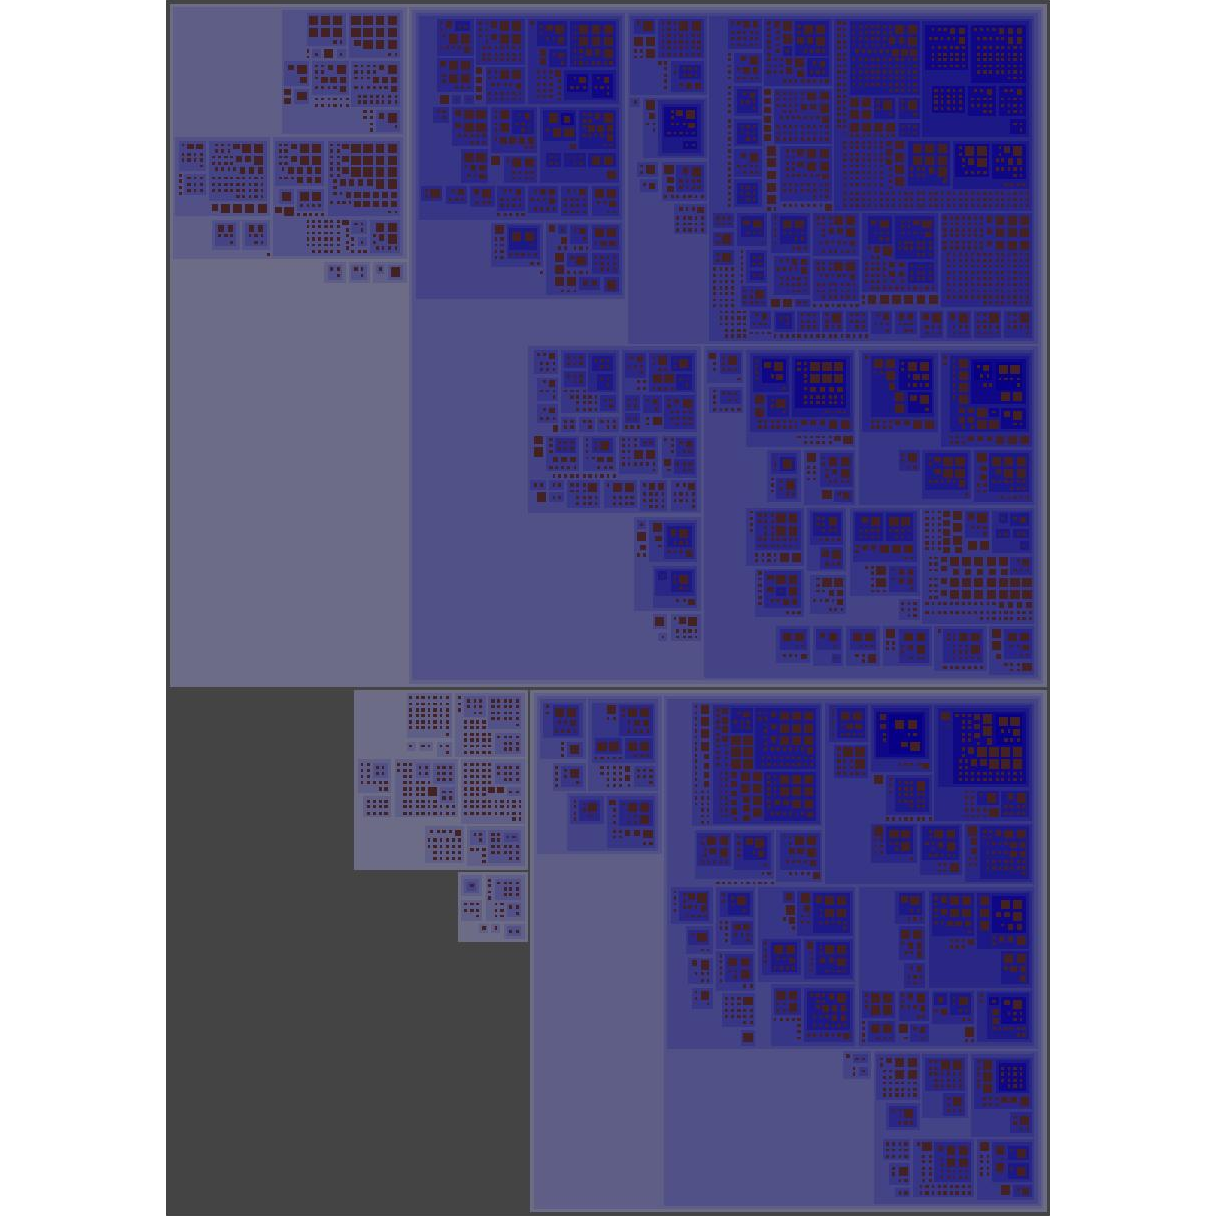
\includegraphics[width=\examplesdefaultwidth]{figures/codecity.png}};
		\node[below=5pt of sot-3,text width=\examplesdefaultwidth,align=center] (sot-3-label) { CodeCity };
		\node[right=10pt of sot-1.south east,anchor=south west] (sot-4) {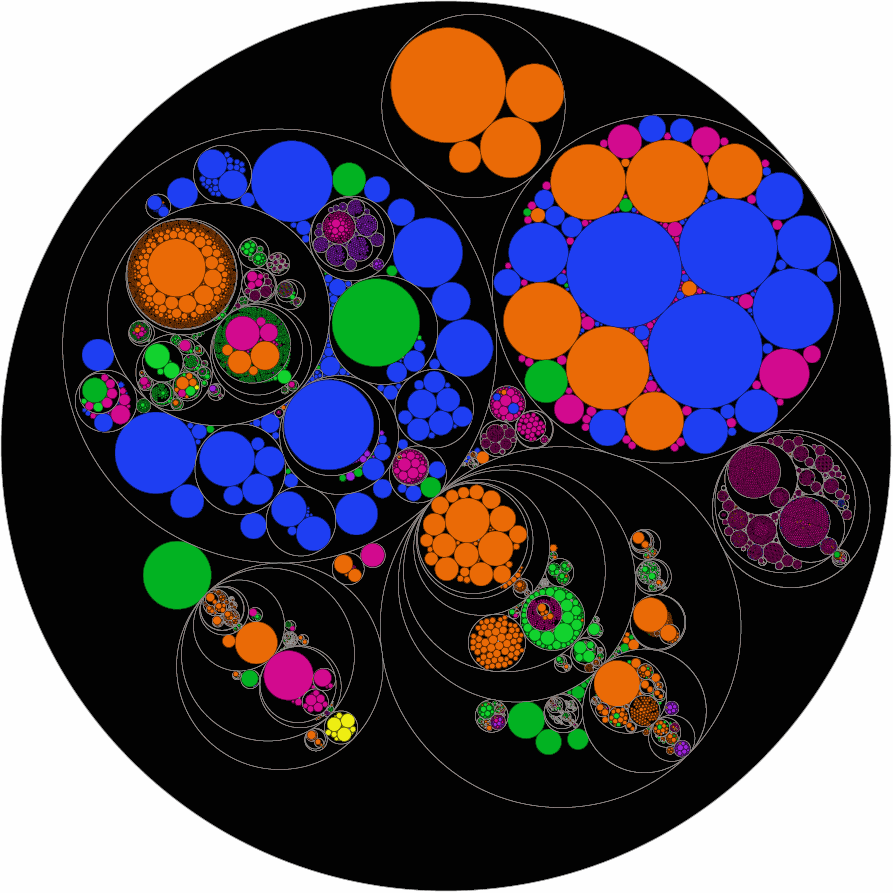
\includegraphics[width=\examplesdefaultwidth]{figures/pebbles.png}};
		\node[below=5pt of sot-4,text width=\examplesdefaultwidth,align=center] (sot-4-label) { Pebbles Treemap };
		\node[right=10pt of sot-4] (sot-5) {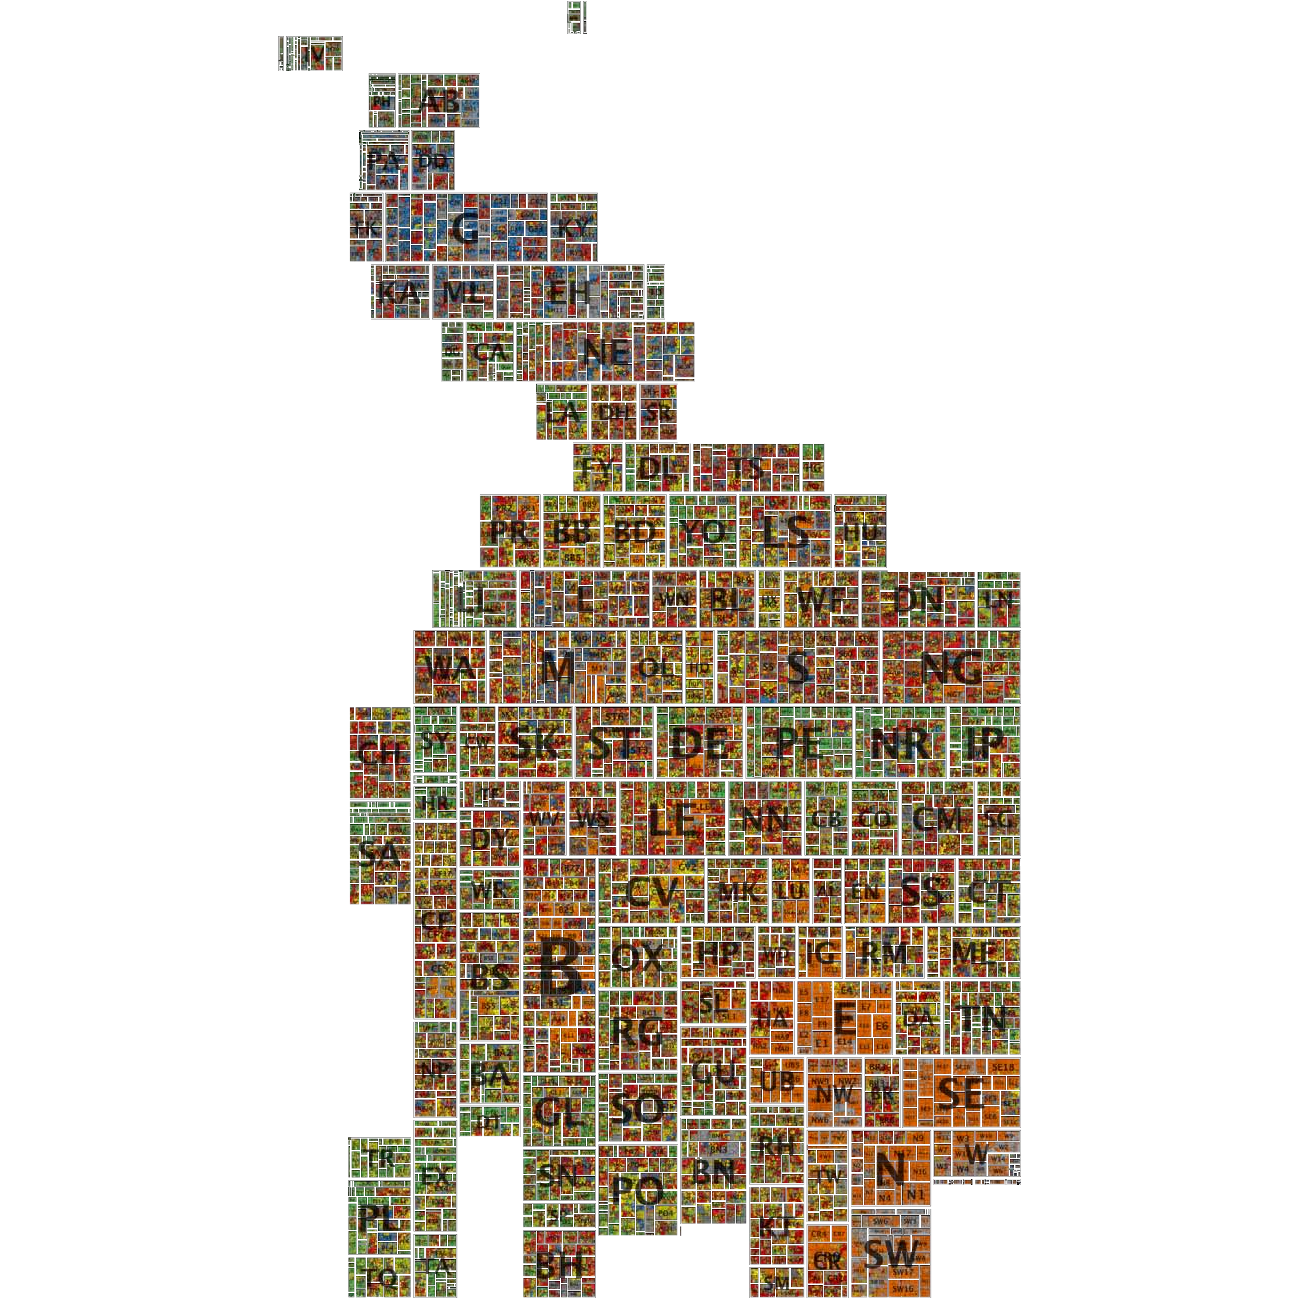
\includegraphics[width=\examplesdefaultwidth]{figures/cartogram.png}};
		\node[below=5pt of sot-5,text width=\examplesdefaultwidth,align=center] (sot-5-label) { Rectangular Hierarchical Cartogram };
		\node[above=5pt of sot-2.north west,xshift=-5pt] (Tc) { \Tc };
		\draw[thin,black,shorten >= 10pt] (Tc-|sot-1.west) -- (Tc);
		\draw[thin,black,shorten <= 10pt] (Tc) -- (Tc-|sot-3.east);
		\end{tikzpicture}
		\caption{Examples of treemaps from the category \emph{Containment Treemap}. Image courtesy from left to right and top to bottom: \cite{itoh2004-reactanglepacking}, \cite{scheibel2018-evocells}, \cite{wettel2007-cities}, \cite{wetzel2003-pebbles}, and \cite{slingsby2010-cartograms}.}
	\end{figure}
\end{frame}

\begin{frame}[c]{Implicit Edge Representation Tree -- \Tie}
	\begin{figure}
		\centering
		\footnotesize
		\begin{tikzpicture}[every node/.style={inner sep=0,outer sep=0},node distance=0pt]
		\node[] (sot-1) {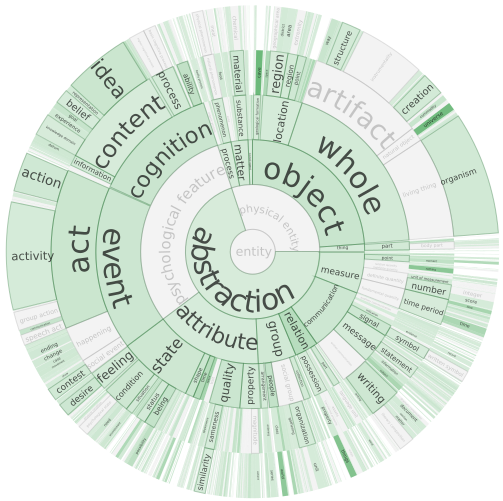
\includegraphics[width=\exampleslargewidth]{figures/sunburst.png}};
		\node[below=5pt of sot-1,text width=0.7\exampleslargewidth,align=center] (sot-1-label) { Sunburst View };
		\node[right=10pt of sot-1.north east,anchor=north west] (sot-2) {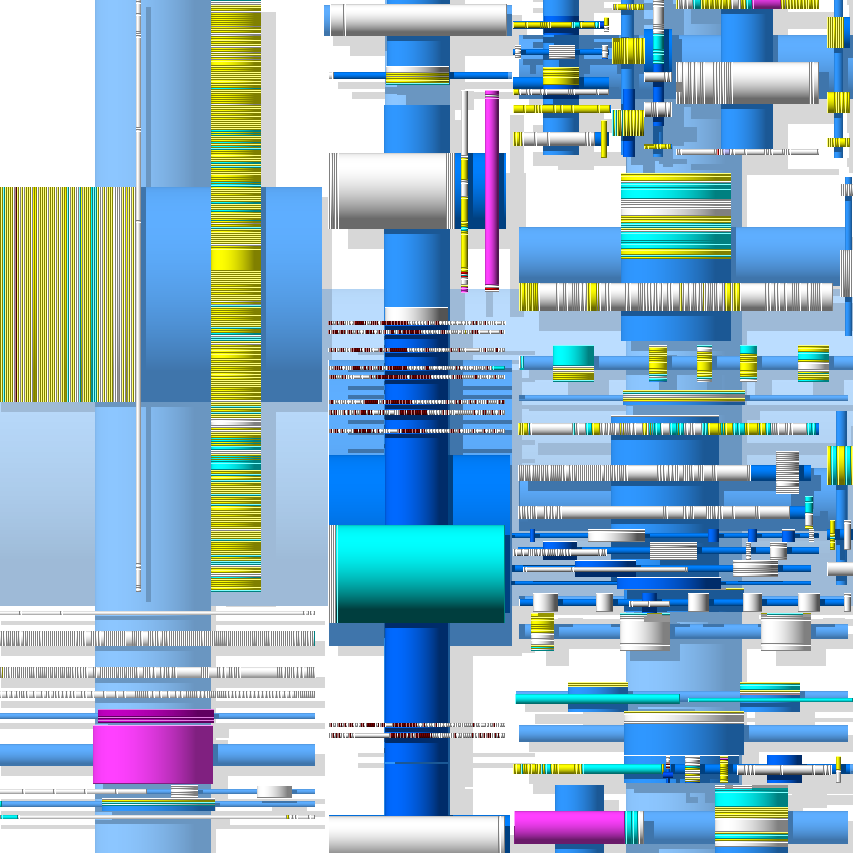
\includegraphics[width=\examplesdefaultwidth]{figures/beamtree-hr.png}};
		\node[below=5pt of sot-2,text width=\examplesdefaultwidth,align=center] (sot-2-label) { BeamTree };
		\node[right=10pt of sot-2] (sot-3) {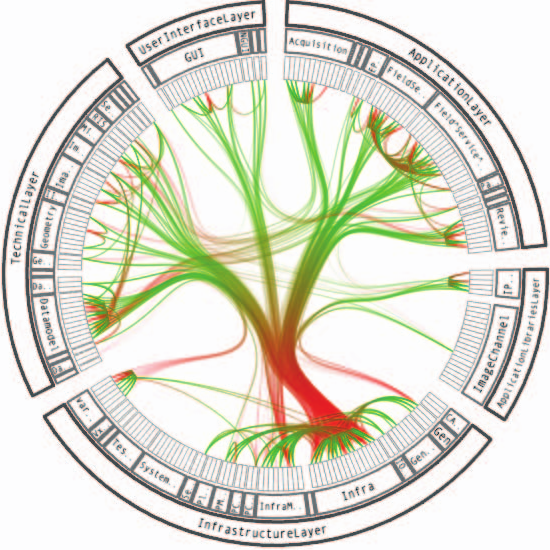
\includegraphics[width=\examplesdefaultwidth]{figures/bundleview.png}};
		\node[below=5pt of sot-3,text width=\examplesdefaultwidth,align=center] (sot-3-label) { Bundle View };
		\node[right=10pt of sot-1.south east,anchor=south west] (sot-4) {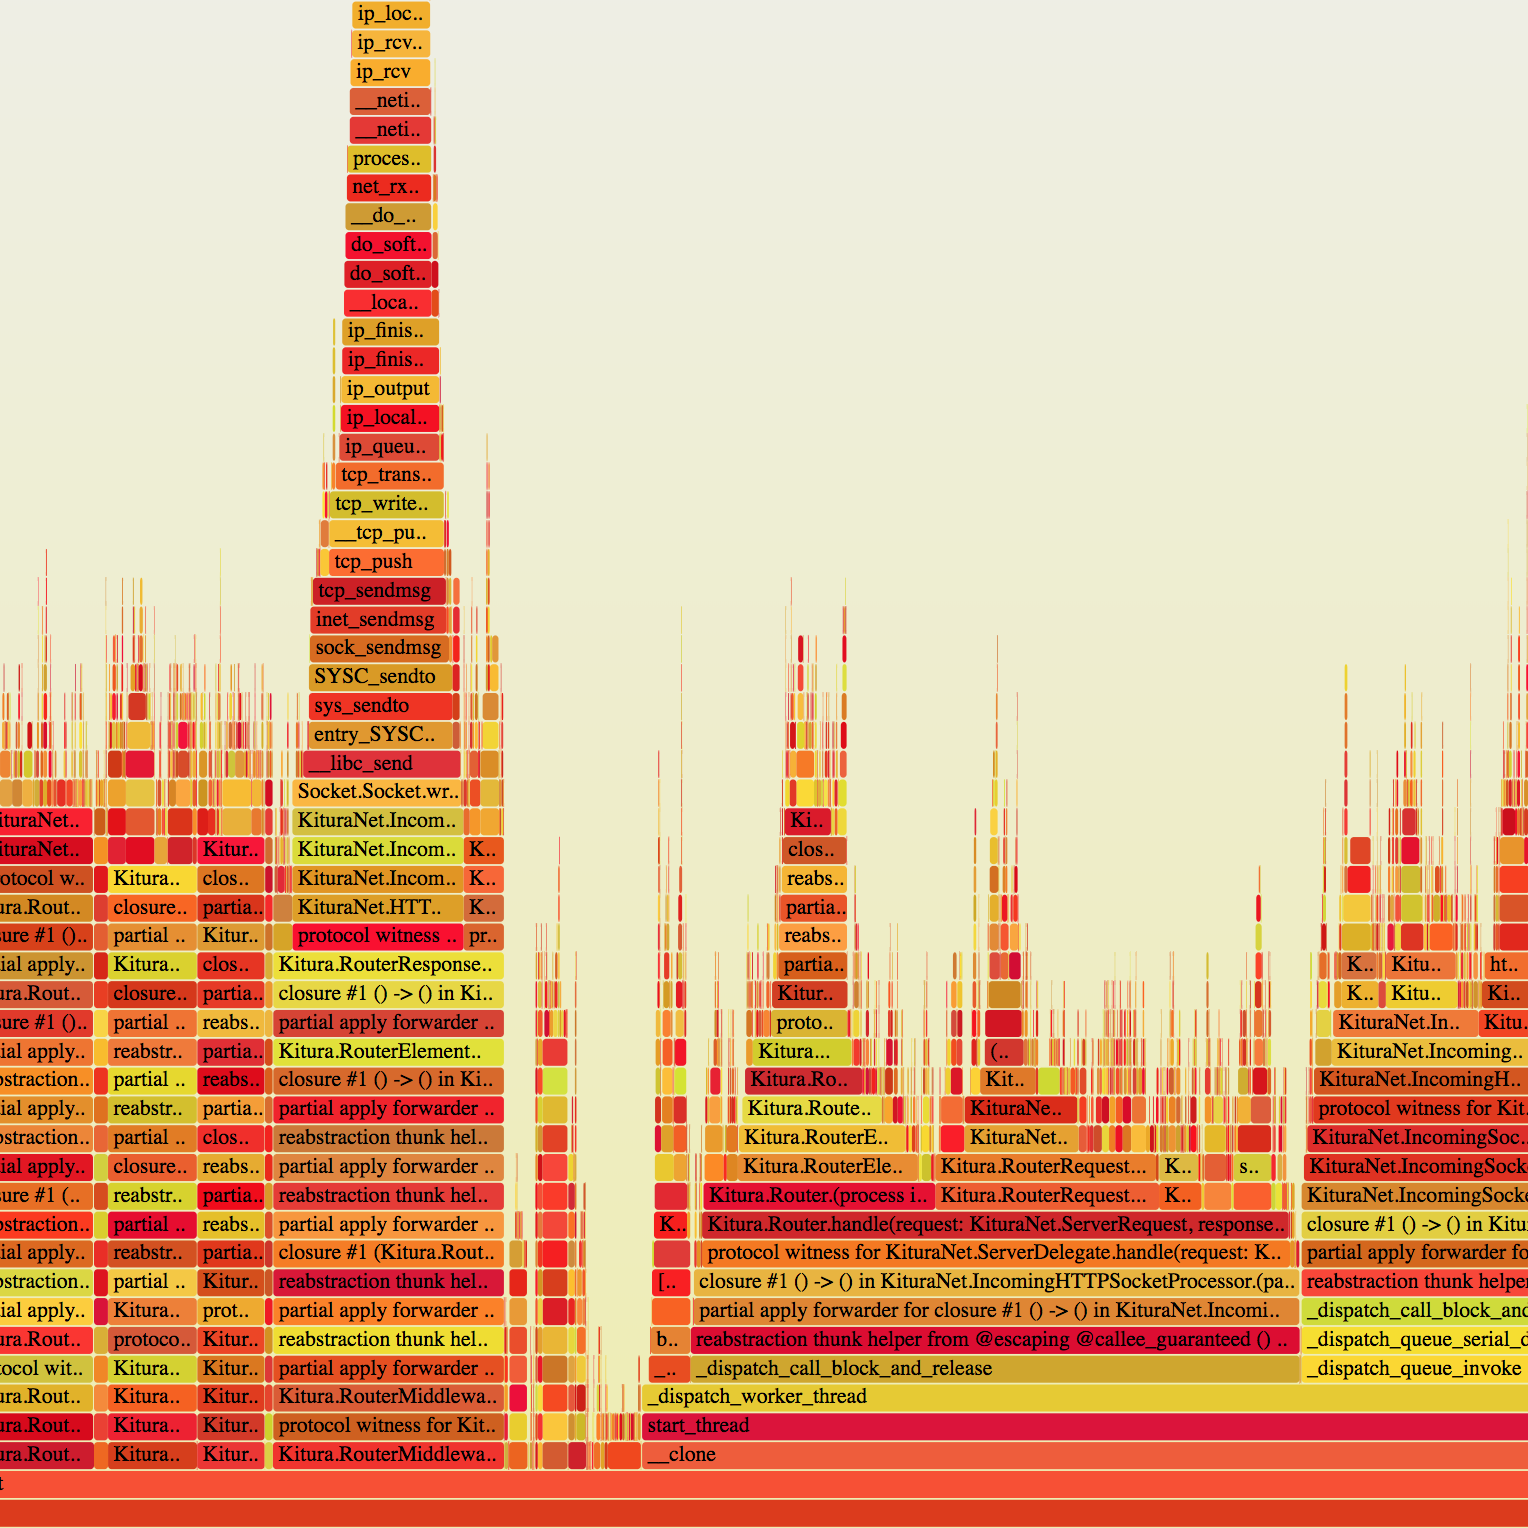
\includegraphics[width=\examplesdefaultwidth]{figures/flamegraph-hr.png}};
		\node[below=5pt of sot-4,text width=\examplesdefaultwidth,align=center] (sot-4-label) { Flame Graphs };
		\node[right=10pt of sot-4] (sot-5) {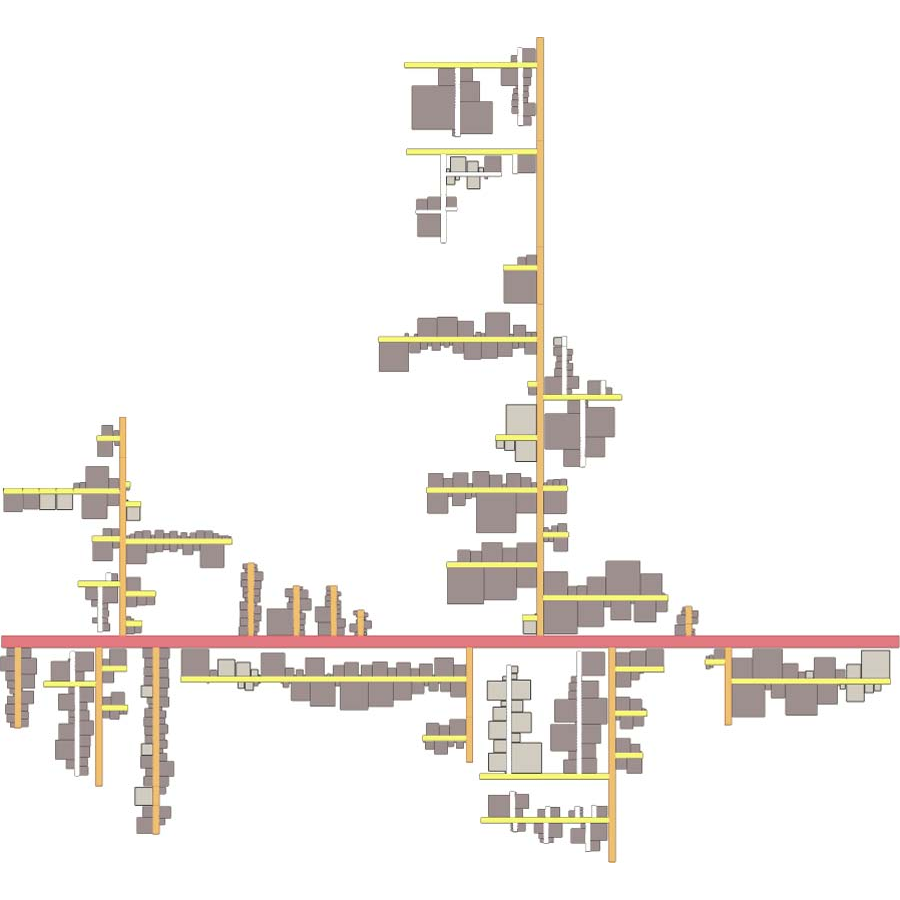
\includegraphics[width=\examplesdefaultwidth]{figures/evostreets.png}};
		\node[below=5pt of sot-5,text width=\examplesdefaultwidth,align=center] (sot-5-label) { Software Cities };
		\node[above=5pt of sot-2.north west,xshift=-5pt] (Tie) { \Tie };
		\draw[thin,black,shorten >= 10pt] (Tie-|sot-1.west) -- (Tie);
		\draw[thin,black,shorten <= 10pt] (Tie) -- (Tie-|sot-3.east);
		\end{tikzpicture}
		\caption{Examples of treemaps from the category \emph{Implicit Edge-Representation Treemap}. Image courtesy from left to right and top to bottom: \cite{stasko2000-structures}, \cite{vanHam2003-beamtrees}, \cite{holten2006-edgebundles}, \cite{gregg2016-flamegraphs}, and \cite{steinbruckner2013-evolution}.}
	\end{figure}
\end{frame}

\begin{frame}[c]{Mapped Tree -- \Tmt}
	\begin{figure}
		\centering
		\footnotesize
		\begin{tikzpicture}[every node/.style={inner sep=0,outer sep=0},node distance=0pt]
		\node[] (sot-1) {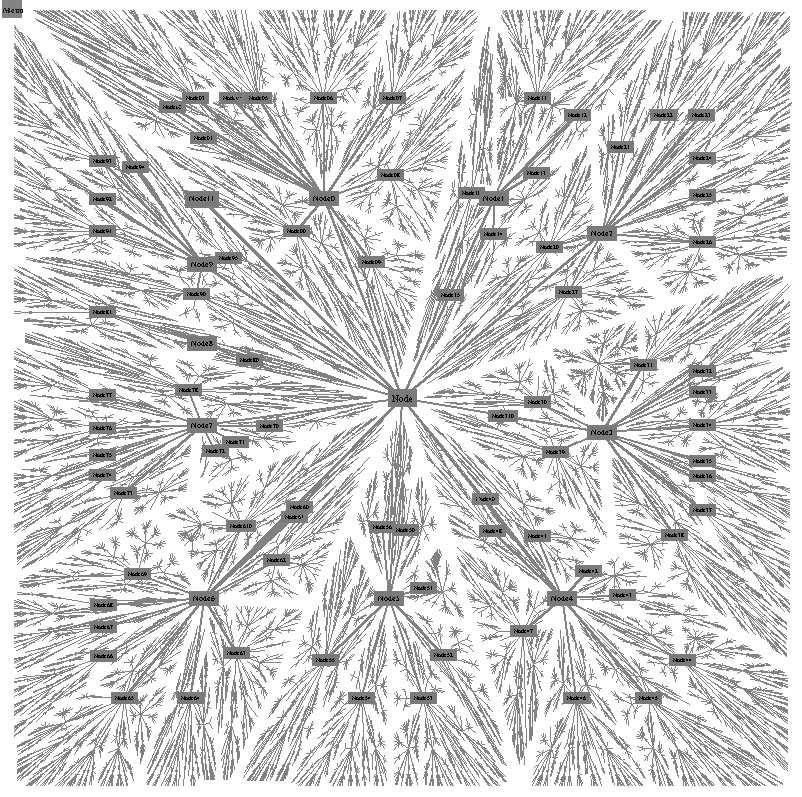
\includegraphics[width=\exampleslargewidth]{figures/spaceoptimizedtree.png}};
		\node[below=5pt of sot-1,text width=0.7\exampleslargewidth,align=center] (sot-1-label) { Space-optimized Tree };
		\node[right=10pt of sot-1.north east,anchor=north west] (sot-2) {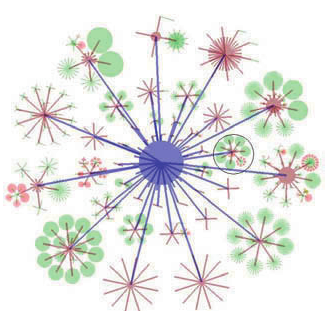
\includegraphics[width=\examplesdefaultwidth]{figures/rings.png}};
		\node[below=5pt of sot-2,text width=\examplesdefaultwidth,align=center] (sot-2-label) { RINGS };
		\node[right=10pt of sot-2] (sot-3) {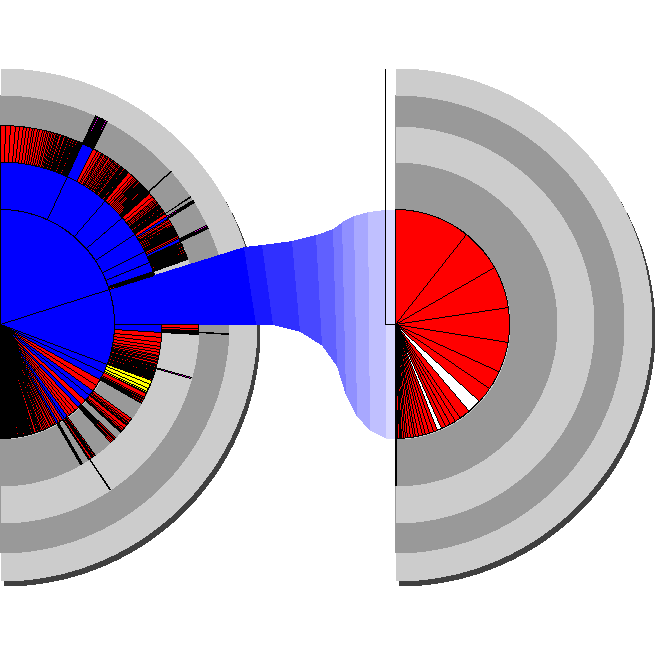
\includegraphics[width=\examplesdefaultwidth]{figures/informationslices.png}};
		\node[below=5pt of sot-3,text width=\examplesdefaultwidth,align=center] (sot-3-label) { Information Slices };
		\node[right=10pt of sot-1.south east,anchor=south west] (sot-4) {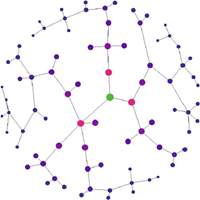
\includegraphics[width=\examplesdefaultwidth]{figures/circular-tree-drawing.png}};
		\node[below=5pt of sot-4,text width=\examplesdefaultwidth,align=center] (sot-4-label) { Tree Drawings };
		\node[right=10pt of sot-4] (sot-5) {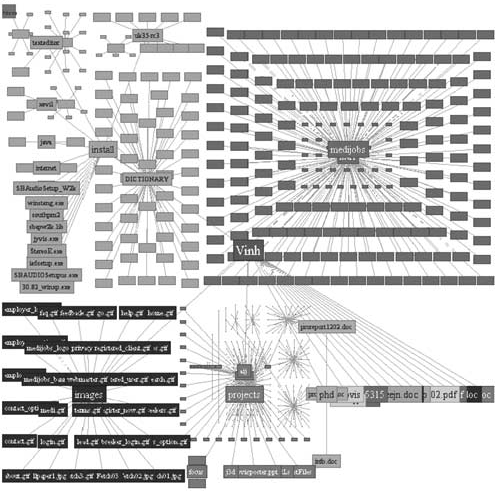
\includegraphics[width=\examplesdefaultwidth]{figures/enccon.png}};
		\node[below=5pt of sot-5,text width=\examplesdefaultwidth,align=center] (sot-5-label) { ENCCON };
		\node[above=5pt of sot-2.north west,xshift=-5pt] (Tmt) { \Tmt };
		\draw[thin,black,shorten >= 10pt] (Tmt-|sot-1.west) -- (Tmt);
		\draw[thin,black,shorten <= 10pt] (Tmt) -- (Tmt-|sot-3.east);
		\end{tikzpicture}
		\caption{Examples of treemaps from the category \emph{Mapped Tree}. Image courtesy from left to right and top to bottom: \cite{nguyen2002-sot}, \cite{teoh2002-rings}, \cite{andrews1998-slices}, \cite{toosi2014-circular}, and \cite{nguyen2005-enccon}.}
	\end{figure}
\end{frame}

\begin{frame}{Taxonomy of Treemap Categories}
	\textbf{Proposed Categories of Treemap Taxonomy}
	\begin{figure}
		
% !TeX root = ../treemap-taxonomy-ivapp2020.tex

%
{%
	%\pfinal
	%\scriptsize%
	\footnotesize
	\centering%
	%\newlength{\definitionswidth}%
	%\newlength{\definitionsoffset}%
	%\newlength{\definitionsimagesize}%
	%\newlength{\definitionsdescriptionsize}%
	\setlength{\definitionswidth}{\textwidth}%
	\setlength{\definitionsoffset}{13pt}%
	\setlength{\definitionsimagesize}{0.25\definitionswidth - 2\definitionsoffset}%
	\setlength{\definitionsdescriptionsize}{0.25\definitionswidth - 0.5\definitionsoffset}%
	\begin{tikzpicture}[]
	% Images
	\node[inner sep=0,outer sep=0] (space-filling) at (-1.5\definitionsimagesize - 3\definitionsoffset, 0.0) {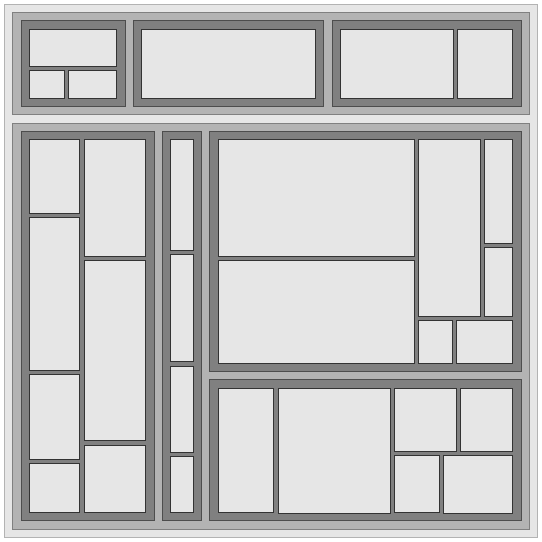
\includegraphics[width=\definitionsimagesize]{figures/treemap-cat-s}};
	\node[inner sep=0,outer sep=0] (containment) at (-0.5\definitionsimagesize + -1\definitionsoffset, 0.0) {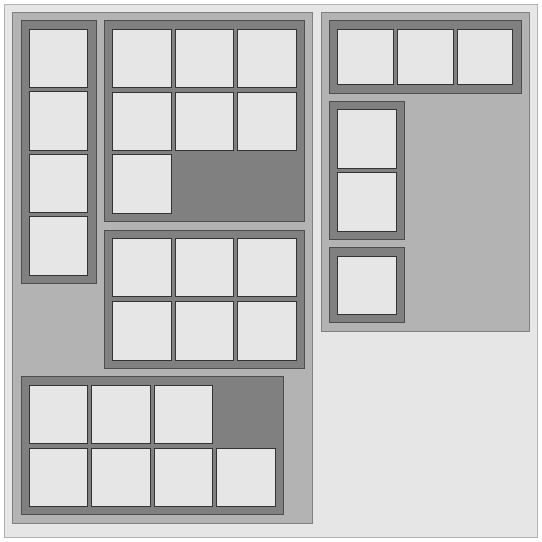
\includegraphics[width=\definitionsimagesize]{figures/treemap-cat-c}};
	\node[inner sep=0,outer sep=0] (implicit-edge) at (0.5\definitionsimagesize + 1\definitionsoffset, 0.0) {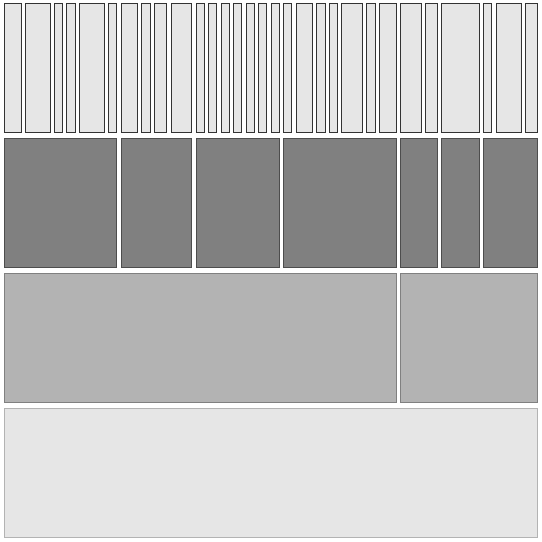
\includegraphics[width=\definitionsimagesize]{figures/treemap-cat-ie}};
	\node[inner sep=0,outer sep=0] (mapped-tree) at (1.5\definitionsimagesize + 3\definitionsoffset, 0.0) {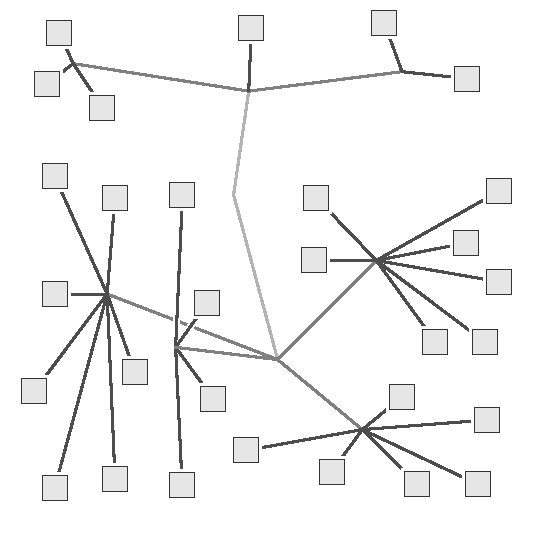
\includegraphics[width=\definitionsimagesize]{figures/treemap-cat-mt}};
	% Labels
	\node[above=0cm of space-filling] (tm0) {\Ts};
	\node[below=0cm of space-filling,text width=\definitionsdescriptionsize,align=center] (tm0-description) { Space-filling Treemap };
	\node[above=0cm of containment] (tm1) {\Tc};
	\node[below=0cm of containment,text width=\definitionsdescriptionsize,align=center] (tm1-description) { Containment Treemap };
	\node[above=0cm of implicit-edge] (tm2) {\Tie};
	\node[below=0cm of implicit-edge,text width=\definitionsdescriptionsize,align=center] (tm2-description) { Implicit Edge Representation Tree };
	\node[above=0cm of mapped-tree] (tm3) {\Tmt};
	\node[below=0cm of mapped-tree,text width=\definitionsdescriptionsize,align=center] (tm3-description) { Mapped Tree };
	\only<2-3|handout:1>{
		% Relations
		\draw[draw=none] (space-filling.east) -- (containment.west) node[pos=0.5] {\huge $\subset$};
		\draw[draw=none] (containment.east) -- (implicit-edge.west) node[pos=0.5] (splitting-subset) {\huge $\subset$};
		\draw[draw=none] (implicit-edge.east) -- (mapped-tree.west) node[pos=0.5] {\huge $\subset$};
	}
	\only<3|handout:1>{
		% Discriminator Line
		\draw[draw=none] (containment.center) -- (splitting-subset.center) node [pos=0.85] (discriminator-x) {};
		\draw[densely dotted,line width=0.75pt,shorten <= 5pt,shorten >= 5pt] (discriminator-x |- tm2.north) -- (discriminator-x |- tm2-description.south);
	}
	\end{tikzpicture}%
}%
%

		\caption{\only<3|handout:1>{The four proposed treemap categories, namely Space-filling Treemap, Containment Treemap, Implicit Edge Representation Tree, and Mapped Tree. Each category includes their predecessors, building a more general category. The dotted line highlights the observed current border, whether a visualization technique is called a treemap.}}
	\end{figure}
\end{frame}
